\subsubsection{\textbf{Tree Edit Distance (TREED)}}  
The sematical quality of translated code depends on its syntax. Until now, abstract syntax trees(AST) are structures widely used in  representing the structure of program code. 

This metric measures the difference between the Abstract Syntax Trees (AST) of referenced method and translated method. Specifically, the tree edit distance between two trees is calculated by number of operations (add/delete/replace/move) to make them identical. \cite{algorithm}. 

It is computed as:  $TREED = 1 -  \frac{TreeEditDistance\left(AST_R, AST_T\right)}{CountNodes \left(AST_R+AST_T\right)}$ where $TreeEditDistance\left(AST_R, AST_T\right)$ is the editing distance between two trees of referenced method $AST_R$ and the translated method $AST_T$; and the denominator is the total nodes in the tree of both two methods. The value of TREED is from 0 to 1. For any two trees, there will always exist at least one editing (such as the one that deletes all nodes of the first tree and inserts all the nodes of the second). Therefore, there will always exist at least one TREED value and the higher value is, the more similar those trees are.

\begin{figure}[h]
	\caption{Tree Editing Example: In the label of each node, its type is in capital font and its val (if exists) is in normal font}
	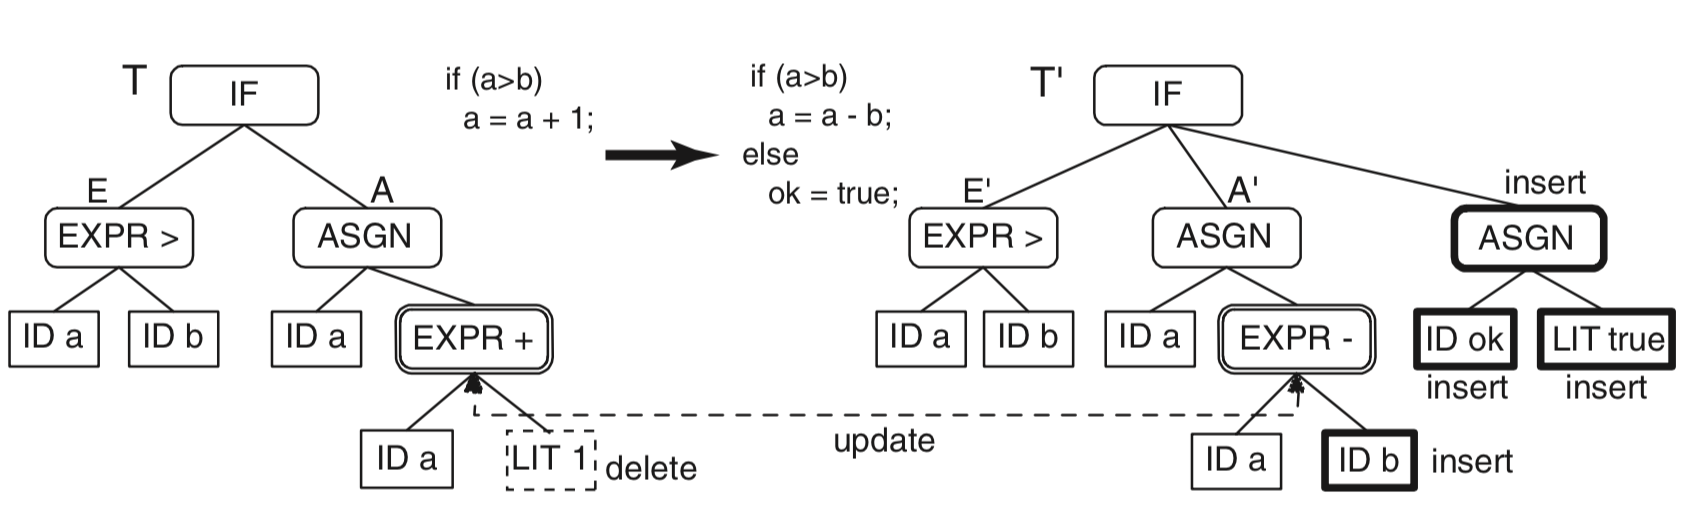
\includegraphics[scale=0.3]{img/treed.png}
	\centering
	\label{fig:treed}
\end{figure}

In the example in Figure 1, an \textit{if} statement was edited by modifying the \textit{if} branch and adding an \textit{else} branch. The two trees represent the two versions of a method. An editing consists of one \textit{Delete} (dotted line box), one \textit{Update} (double-line box), and four \textit{Insert} operations (bold boxes). Other nodes (single- line boxes) are either unchanged or moved. Based on the formula TREED, the result of TREED in this case  $TREED = 1 - \frac{1 + 1 + 4}{16}=0.625$



